%%%%%%%%%%%%%%%%%%%%%%%%%%%%%%%%%%%%%%%%%
% a0poster Portrait Poster
% LaTeX Template
% Version 1.0 (22/06/13)
%
% The a0poster class was created by:
% Gerlinde Kettl and Matthias Weiser (tex@kettl.de)
% 
% This template has been downloaded from:
% http://www.LaTeXTemplates.com
%
% License:
% CC BY-NC-SA 3.0 (http://creativecommons.org/licenses/by-nc-sa/3.0/)
%
%%%%%%%%%%%%%%%%%%%%%%%%%%%%%%%%%%%%%%%%%

%----------------------------------------------------------------------------------------
%	PACKAGES AND OTHER DOCUMENT CONFIGURATIONS
%----------------------------------------------------------------------------------------

\documentclass[a0,portrait]{a0poster}

\usepackage{multicol} % This is so we can have multiple columns of text side-by-side
\columnsep=100pt % This is the amount of white space between the columns in the poster
\columnseprule=3pt % This is the thickness of the black line between the columns in the poster

\usepackage[svgnames]{xcolor} % Specify colors by their 'svgnames', for a full list of all colors available see here: http://www.latextemplates.com/svgnames-colors

\usepackage{times} % Use the times font
%\usepackage{palatino} % Uncomment to use the Palatino font
\usepackage{makecell}                 % 三线表-竖线
\usepackage{booktabs}                 % 三线表-短细横线
\usepackage{graphicx}				  % 表格单元格逆时针
\usepackage{multirow}				  % 合并单元格
\usepackage{array}
\usepackage{amssymb}				  % 勾
\usepackage{longtable}                % 导入 longtable 宏包,表格自动换行
\usepackage{amsmath}
\usepackage{graphicx} % Required for including images
\graphicspath{{figures/}} % Location of the graphics files
\usepackage{booktabs} % Top and bottom rules for table
\usepackage[font=small,labelfont=bf]{caption} % Required for specifying captions to tables and figures
\usepackage{amsfonts, amsmath, amsthm, amssymb} % For math fonts, symbols and environments
\usepackage{wrapfig} % Allows wrapping text around tables and figures
\usepackage{graphicx}
\usepackage{caption}
\usepackage{subcaption}
\usepackage[final]{hyperref} % adds hyper links inside the generated pdf file
\hypersetup{
	colorlinks=true,       % false: boxed links; true: colored links
	linkcolor=blue,        % color of internal links
	citecolor=blue,        % color of links to bibliography
	filecolor=magenta,     % color of file links
	urlcolor=blue         
}


\begin{document}

%----------------------------------------------------------------------------------------
%	POSTER HEADER 
%----------------------------------------------------------------------------------------

% The header is divided into two boxes:
% The first is 75% wide and houses the title, subtitle, names, university/organization and contact information
% The second is 25% wide and houses a logo for your university/organization or a photo of you
% The widths of these boxes can be easily edited to accommodate your content as you see fit

\begin{minipage}[b]{0.75\linewidth}
\Huge \color{NavyBlue} \textbf{Anomaly detection of multicariate time series} \color{Black}\\ % Title
\LARGE \textit{An improved method for multivariate time series under cdn network}\\[2cm] % Subtitle
\LARGE \textbf{Wang Zhong, Gu Rui, Pan Zhongli}\\[0.5cm] % Author(s)
\LARGE LanZhou University, IC@PS\\ [0.4cm] % University/organization
\large Lanzhou University Annual meeting paper 
\\
\end{minipage}
%
\hspace{-5.5cm}\begin{minipage}[b]{0.3\linewidth}
% \includegraphics[scale=0.5]{ciencias.png}\qquad

\includegraphics[scale=2.5]{lzu.png}
\end{minipage}

\vspace{1cm} % A bit of extra whitespace between the header and poster content

%----------------------------------------------------------------------------------------

\begin{multicols}{2} % This is how many columns your poster will be broken into, a portrait poster is generally split into 2 columns

%----------------------------------------------------------------------------------------
%	ABSTRACT
%----------------------------------------------------------------------------------------


\color{DarkRed}

\begin{abstract}
	This paper summarizes CDN KPI anomaly detection algorithms and their evaluation methods. Different websites' KPIs exhibit distinct structures and non-stationary relationships over time, posing a challenge for deep learning approaches. To address this, we propose an improved method.
\end{abstract}

%----------------------------------------------------------------------------------------
%	INTRODUCTION
%----------------------------------------------------------------------------------------

\color{Black}
\section*{Introduction}

\quad With the growth of Internet companies, traditional methods face challenges in detecting KPI exceptions, and machine learning-based CDN KPI abnormal detection is essential\cite{b1}. CDN operators collect various KPIs, and the Fig.\ref{fig: Abnormal Data} shows an example. Deep anomaly detection uses RNN for feature extraction, but current methods cannot handle non-stationary dependencies and multi-website anomalies effectively.

\begin{center}\vspace{1cm}
	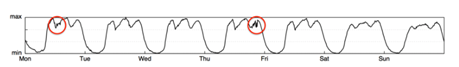
\includegraphics[width=0.8\linewidth]{abnormal_data}
	\captionof{figure}{
		\label{fig: Abnormal Data}
		The amount of data visited on the network page of an Internet company was abnormal}
\end{center}\vspace{1cm}

%----------------------------------------------------------------------------------------
%	CHALLENGE
%----------------------------------------------------------------------------------------


\section*{Challenge}

\quad \textit{Challenge 1}: Non-stationary dependencies between time periods degrade deep anomaly detection models. Fig.\ref{fig: CDN KPIs of 6-websites}(a) and Fig.\ref{fig: CDN KPIs of 6-websites}(d) show different user request behavior on weekdays vs. weekends. KPI changes during scheduled node sets, as shown in Fig.\ref{fig: CDN KPIs of 6-websites}(b), resulting in non-stationary temporal characteristics. Current methods struggle to capture expected patterns, leading to inferior performance in anomaly detection for CDNs.

\begin{center}\vspace{1cm}
	
	\begin{minipage}[c]{0.18\linewidth}	
		\centering
		\captionsetup[subfigure]{labelformat=parens} % 设置子图类型为圆括号
		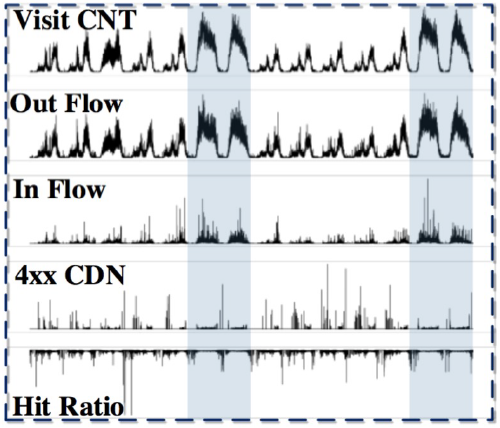
\includegraphics[width=\linewidth]{CDN_KPI/cdn_kpi_a}
		\captionof*{figure}{(a)}
		\label{fig:cdn_kpi_a}
	\end{minipage}
	\begin{minipage}[c]{0.18\linewidth}
		\centering
		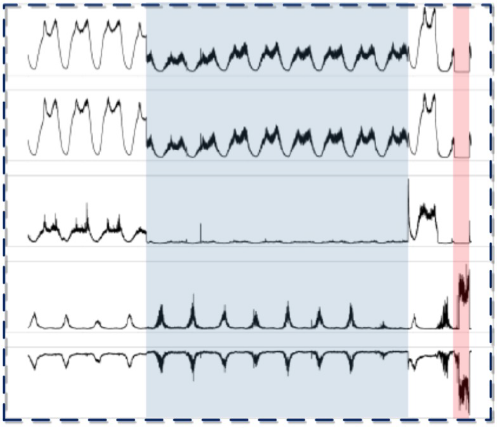
\includegraphics[width=\linewidth]{CDN_KPI/cdn_kpi_b}
		\captionof*{figure}{(b)}
		\label{fig:cdn_kpi_b}
	\end{minipage}
	\begin{minipage}[c]{0.18\linewidth}
		\centering
		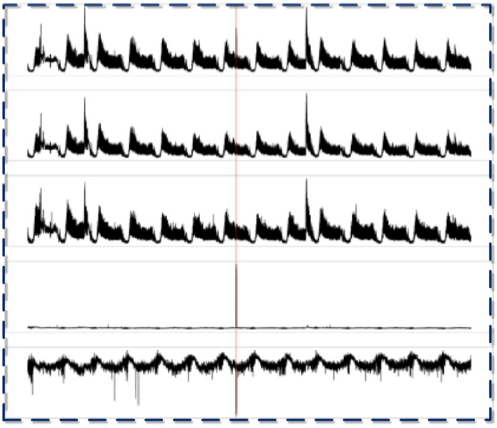
\includegraphics[width=\linewidth]{CDN_KPI/cdn_kpi_c}
		\captionof*{figure}{(c)}
		\label{fig:cdn_kpi_c}
	\end{minipage}\\
	\begin{minipage}[c]{0.18\linewidth}
		\centering
		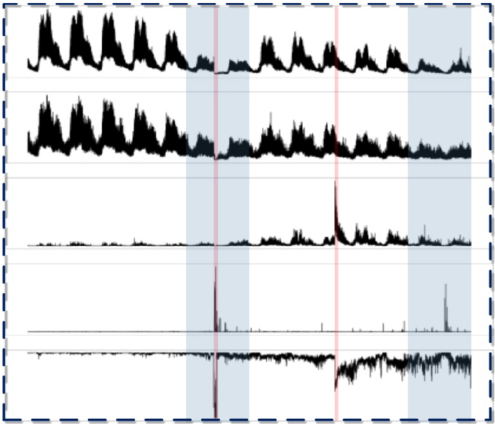
\includegraphics[width=\linewidth]{CDN_KPI/cdn_kpi_d}
		\captionof*{figure}{(d)}
		\label{fig:cdn_kpi_d}
	\end{minipage}
	\begin{minipage}[c]{0.18\linewidth}
		\centering
		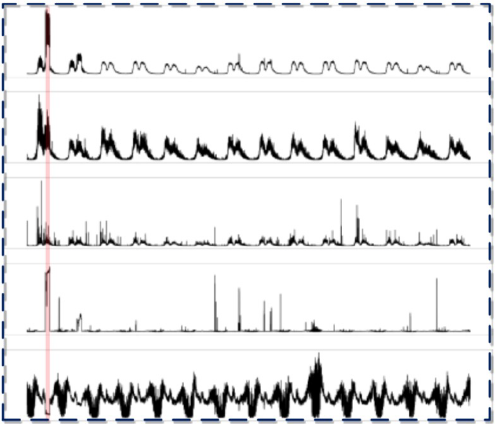
\includegraphics[width=\linewidth]{CDN_KPI/cdn_kpi_e}
		\captionof*{figure}{(e)}
		\label{fig:cdn_kpi_e}
	\end{minipage}
	\begin{minipage}[c]{0.18\linewidth}
		\centering
		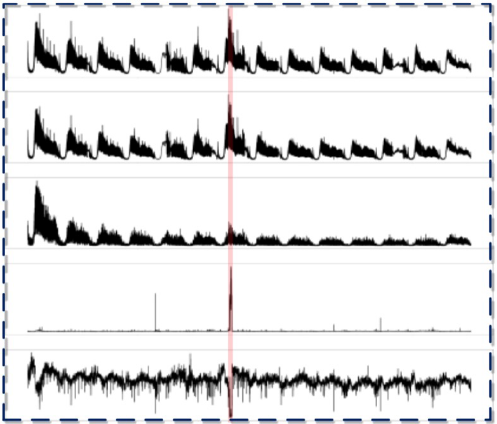
\includegraphics[width=\linewidth]{CDN_KPI/cdn_kpi_f}
		\captionof*{figure}{(f)}
		\label{fig:cdn_kpi_f}
	\end{minipage} 
		\captionof{figure}{
			\label{fig: CDN KPIs of 6-websites}
			2-weeks real world typical multivariate CDN KPIs of 6-websites. Periods in light blue show the change points in KPIs; Regions highlighted in red represent the ground-truth
			anomaly segments.
		}

\end{center}\vspace{1cm}

\textit{Challenge 2}: CDNs provide services for a diverse set of websites, but current deep anomaly detection models struggle to capture the dynamic complexity of these websites in one model. Training an individual model for each website consumes a lot of resources and raises maintenance costs. Additionally, KPIs of different websites may exhibit similar characteristics, rendering individual models for each website unnecessary.

%----------------------------------------------------------------------------------------
%	MATERIALS AND METHODS
%----------------------------------------------------------------------------------------

\section*{Methods}

\quad CDN KPIs are denoted by $x_n$, where $n=1,...,N$ and $N$ is the number of KPI time series. The observation at time $t$ is $x_{t,n}\in \mathbb{R}^V$, a $V$-dimensional vector, thus $x_n\in \mathbb{R}^{T\times V}$, where $T$ is the duration of $x_n$. Anomaly detection on CDN KPIs aims to determine whether $x_{t,n}$ is anomalous or not for a given website. To achieve unsupervised anomaly detection, robust representations of the input data need to be learned using an efficient method.

\subsection*{Variational RNN (VRNN)}

\quad The VRNN\cite{b4} has VAE\cite{b5} at each timestep, conditioned on the last timestep's latent states. The prior on latent variables is not standard Gaussian as assumed in VAE, but follows a specific distribution.
\begin{equation}
	\begin{gathered}
		z_{t} \sim \mathcal{N}\left(\mu_{0,t},\text{diag}(\sigma_{0,t}^{2})\right), \\
		\left[\mu_{0,t},\sigma_{0,t}\right]=\varphi_{\tau}^{\text{dec}}\left(\varphi_{\tau}^z {(z_t)},h_{t-1}\right)
	\end{gathered}
\end{equation}

The generating distribution of the VRNN is conditioned on both the latent variable $z_t$ and the hidden state variable $h_{t-1}$ as

\begin{equation}
	\begin{gathered}
		x_t | z_t \sim \mathcal{N}\left(\mu_{x,t}, \text{diag}(\sigma_{x,t}^{2})\right), \\
		\left[ \mu_{x,t} , \sigma_{x,t} \right] = \varphi_{\tau}^\text{dec} \left( \varphi_\tau^{z}(z_t),h_{t-1}\right)
	\end{gathered}
\end{equation}

To infer $z_t$, like standard VAE, a Gaussian distributed variational distribution $q(z_t|x_t)$ is used to approximate its true posterior. In a similar fashion with the generative process of VRNN, the variational distribution is a function of both $x_t$ and $h_{t-1}$ as

\begin{equation}
	\begin{gathered}
		z_t | x_t \sim \mathcal{N}\left(\mu_{x,t}, \text{diag}(\sigma_{z,t}^{2})\right), \\
		\left[ \mu_{z,t} , \sigma_{z,t} \right] = \varphi_{\tau}^\text{enc} \left( \varphi_\tau^{x}(x_t),h_{t-1}\right)
	\end{gathered}
\end{equation}

%------------------------------------------------

\subsection*{Our Methods}

\quad To model the data diversity at different timesteps of multivariate CDN KPIs and solve the non-stationary temporal dependence between them, we extend VRNN into SGmVRNN. Specifically, unlike the standard VRNN, we introduce latent discrete variable $c_{t,n}$ and assign the form of the prior of the latent random variable as

\begin{equation}
	z_{t,n} |c_{t,n} \sim \prod_{k=1}^{K} \mathcal{N}\left(z_{t,n} | \mu_k, \text{diag}(\sigma_{k})\right)^{c_{t,n,k}}
\end{equation}

In this way, we assign a different Gaussian distributed prior conditioned on $c_{t,n}$ for latent variable $z_{t,n}$ at different timesteps, which indicates the diverse distribution characteristics of input. Moreover, marginalizing $c_{t,n}$, we can achieve

\begin{equation}
	z_{t,n} \sim \sum_{c_{t,n}} p\left(c_{t,n}|\pi_{t.n}\right) p\left(z_{t,n} | c_{t,n}\right) = \sum_{k=1}^K \pi_{t,n,k} \mathcal{N}\left(\mu_k, \text{diag}(\sigma_{k})\right)
\end{equation}

Clearly, it is mixture Gaussian distribution with higher representation power than a Gaussian distribution, and thus is just
ideal for characterizing the complex structure and temporal
characteristics within multivariate CDN KPIs.

%----------------------------------------------------------------------------------------
%	MODEL TRAINING
%----------------------------------------------------------------------------------------
\section*{Model Training}

Our training objective is to minimize the distance between the variational distribution of latent variables $q\left(z_{t,n},c_{t,n}\right)$ and their true posterior distribution $p(z_{t,n}, c_{t,n}| - )$, which can be quantified by the Kullback-Leibler (\text{KL}) divergence, $\text{KL}\left(q(x)||p(x)\right) = \int q(x) \log \frac{q(x)}{p(x)}dx$. So, during the inference of objective, we aim to minimize $\text{KL}\left(q(z_{t,n}, c_{t,n})||p({z_{t,n},c_{t,n}}|-)\right)$. Following the usual strategy of VAE, we can transfer this KL divergence as

\begin{equation}
	\begin{aligned}
		&\text{KL} \left(q(z_{t,n}, c_{t,n})||p\left(z_{t,n}, c_{t,n}|- \right)\right) \\
		&= \log p(x_{t,n}) - \mathbb{E}_{q(z_{t,n})q(c_{t,n})} \left(\log p(x_{t,n}|z_{t,n}, c_{t,n}) - \log \frac{q(z_{t,n})q(c_{t,n})}{p(z_{t,n}|c_{t,n})p(c_{t,n})}\right)  \\
		&= \log p(x_{t,n}) - \text{ELBO}
	\end{aligned}
\end{equation}

%----------------------------------------------------------------------------------------
%	ANOMALY DETECTION 
%----------------------------------------------------------------------------------------
\section*{Anomaly Detection}

We apply the reconstruction probability of xt as the anomaly score to determine whether an observed variable is anomalous or not\cite{b3}, and it is computed as

\begin{equation}
	\begin{aligned}
		S_{t,n} = \log p(x_{t,n}|z_{t,n})
	\end{aligned}
\end{equation}


An observation $x_t$ will be classified as anomalous if $S_t$ is below a specific threshold. 


%----------------------------------------------------------------------------------------
%	RESULTS 
%----------------------------------------------------------------------------------------

\section*{Results}

\quad Evaluate our method with "one model for one website" and "one model fits all" experiments. Results in Table\ref{tab: one model fits all websites}, highlighting best F1-score for each dataset.


\begin{center}\vspace{1cm}
	\begin{tabular}{>{\centering\arraybackslash}m{5cm}|>{\centering\arraybackslash}m{2.5cm}>{\centering\arraybackslash}m{2.5cm}>{\centering\arraybackslash}m{2.5cm}|>{\centering\arraybackslash}m{2.5cm}>{\centering\arraybackslash}m{2.5cm}>{\centering\arraybackslash}m{2.5cm}}
		
		\hline %添加表格头部粗线
		
		% \multirow{2}*{\textbf{Learning}} & \multirow{2}*{\textbf{Mathod}} & \multicolumn{4}{c|}{\textbf{LOL-test}} & \multicolumn{4}{c}{\textbf{MIT-Adobe FiveK-test}} \\
		
		\multirowcell{2}{\textbf{Method}} & \multicolumn{3}{c|}{\makecell{\textbf{CDN}}} & \multicolumn{3}{c}{\makecell{\textbf{SMD}}} \\
		
		\cline{2-7}
		
		
		& \textbf{P}  & \textbf{R} & \textbf{F1} & \textbf{P} & \textbf{R}  & \textbf{F1}\\
		
		\hline	
		
		VRNN & 0.9814 & 0.8317 & 0.9003 & 0.9825 & 0.8383 & 0.9047 \\
		DOMI & 0.9665 & 0.8348 & 0.8958 & 0.9770 & 0.8036 & 0.8819 \\
		OmniAnomaly & 0.8385 & 0.8757 & 0.8567 & 0.9801 & 0.7843 & 0.8713 \\
		SDFVAE & 0.9675 & 0.8615 & \underline{0.9115} & 0.9810 & 0.8498 & \underline{0.9107} \\
		
		\hline
		
		SGmVRNN & 0.9667 & 0.9204 & \textbf{0.9430} & 0.9607 & 0.9123 & \textbf{0.9356} \\	
		
		\hline
		
	\end{tabular}
	\captionof{table}{
		\label{tab: one model fits all websites}
		Performance of “one model fits all websites”.}
\end{center}\vspace{1cm}

\begin{center}\vspace{1cm}
	
	\begin{minipage}[c]{0.18\linewidth}	
		\centering
		\captionsetup[subfigure]{labelformat=parens} % 设置子图类型为圆括号
		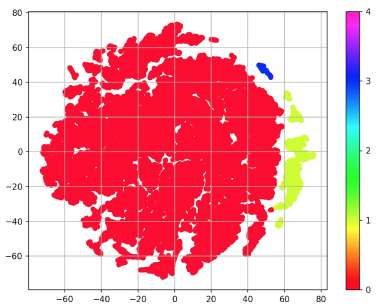
\includegraphics[width=\linewidth]{latent_variables/a}
		\captionof*{figure}{(a)}
		\label{fig: latent_variables_a}
	\end{minipage}
	\begin{minipage}[c]{0.18\linewidth}
		\centering
		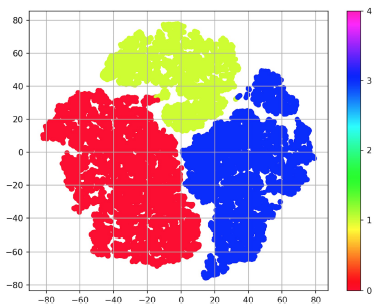
\includegraphics[width=\linewidth]{latent_variables/b}
		\captionof*{figure}{(b)}
		\label{fig: latent_variables_b}
	\end{minipage}
	\begin{minipage}[c]{0.18\linewidth}
		\centering
		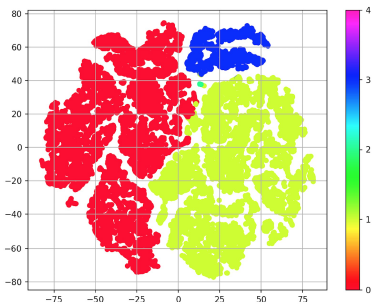
\includegraphics[width=\linewidth]{latent_variables/c}
		\captionof*{figure}{(c)}
		\label{fig: latent_variables_c}
	\end{minipage}
	\begin{minipage}[c]{0.18\linewidth}
		\centering
		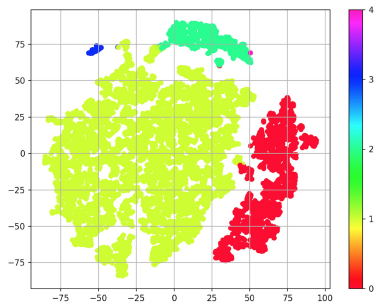
\includegraphics[width=\linewidth]{latent_variables/d}
		\captionof*{figure}{(d)}
		\label{fig: latent_variables_d}
	\end{minipage}
		\captionof{figure}{
		\label{fig: latent variables}
		The visualization of latent variables $z_{t,n}$}
\end{center}\vspace{1cm}

In Fig.\ref{fig: latent variables}, each dot represents a latent variable of an observation at a timestep and colors represent clustering groups. Our model can separate KPIs with different structural characteristics into different groups, which confirms the two challenges mentioned and validates our model's effectiveness.

%----------------------------------------------------------------------------------------
%	CONCLUSIONS
%----------------------------------------------------------------------------------------

\section*{Conclusion}

\begin{itemize}
\item we propose a method to cope with the anomaly detection challenges that brought by the natural characteristics of multivariate CDN KPIs of diverse websites.
\end{itemize}

%----------------------------------------------------------------------------------------
%	REFERENCES
%----------------------------------------------------------------------------------------

\begin{thebibliography}{00}
	
	\bibitem{b1}\label{cite:b1}
		Behrouz Zolfaghari, Gautam Srivastava, Swapnoneel Roy, Hamid R. Nemati, Fatemeh Afghah, Takeshi Koshiba, Abolfazl Razi, Khodakhast Bibak, Pinaki Mitra, and Brijesh Kumar Rai. 2020. Content Delivery Networks: State of the Art, Trends, and Future Roadmap. ACM Comput. Surv. 53, 2, Article 34 (March 2021), 34 pages. https://doi.org/10.1145/3380613	
	\bibitem{b2}\label{cite:b2}
		D. Li, D. Chen, B. Jin, L. Shi, J. Goh, and S. Ng, “MAD-GAN:
		multivariate anomaly detection for time series data with generative adversarial networks,” in Artificial Neural Networks and Machine Learning
		- ICANN, 2019, pp. 703–716
	\bibitem{b3}\label{cite:b3}	
		Y. Su, Y. Zhao, C. Niu, R. Liu, W. Sun, and D. Pei, “Robust anomaly
		detection for multivariate time series through stochastic recurrent neural
		network,” in ACM SIGKDD, 2019, pp. 2828–2837.	
	\bibitem{b4}\label{cite:b4}
		C. Junyoung, K. Kyle, D. Laurent, G. Kratarth, C. C. Aaron, and
		B. Yoshua, “A recurrent latent variable model for sequential data,” in
		NeurIPS, 2015, pp. 2980–2988.
	\bibitem{b5}\label{cite:b5}
		P. K. Diederik and W. Max, “Auto-encoding variational bayes,” in ICLR,
		2014.
		
\end{thebibliography}


\end{multicols}
\end{document}